% Created 2022-04-01 sex 23:47
% Intended LaTeX compiler: pdflatex
\documentclass[11pt]{article}
\usepackage[utf8]{inputenc}
\usepackage[T1]{fontenc}
\usepackage{graphicx}
\usepackage{longtable}
\usepackage{wrapfig}
\usepackage{rotating}
\usepackage[normalem]{ulem}
\usepackage{amsmath}
\usepackage{amssymb}
\usepackage{capt-of}
\usepackage{hyperref}
\usepackage{amsthm}

\theoremstyle{definition}
\newtheorem{teo}{Teorema}[section]
\theoremstyle{definition}
\newtheorem{defi}{Definicao}[section]
\theoremstyle{remark}
\newtheorem{obs}{Observação}[section]
\theoremstyle{remark}
\newtheorem{lema}{Lema}[section]
\theoremstyle{remark}
\newtheorem{prop}{Propriedade}[section]
\theoremstyle{remark}
\newtheorem{coro}{Corolario}[section]
\theoremstyle{definition}
\newtheorem{prep}{Preposição}[section]
\author{Ieremies Romero}
\date{}
\title{MO824 - Atividade 1}
\hypersetup{
 pdfauthor={Ieremies Romero},
 pdftitle={MO824 - Atividade 1},
 pdfkeywords={},
 pdfsubject={},
 pdfcreator={Emacs 27.2 (Org mode 9.6)}, 
 pdflang={Portuguese}}
\usepackage{biblatex}
\addbibresource{~/arq/bib.bib}
\begin{document}

\maketitle

\section*{Formulation}
\label{sec:org756f348}
\subsection*{Objective Function}
\label{sec:org806f9ba}
Our objective, as said in the activity, is to minimize the costs of production and shipment of goods from a set of factories to another set of clients. Since we have cost associated with each of those operations, we will utilize two set of variables: \(x_{p,l,f}\) to represent the amount (in tons) of product \(p \in P\) produced by machine \(l \in L\) at factory \(f \in F\) and \(y_{p, f, j}\) to represent the amount (in tons) of product \(p \in P\) transported from factory \(f \in F\) to client \(j \in J\).

That way, we can describe our objective function as
\[ \min z = \sum \limits_{p \in P} \sum_{f \in F} (\sum \limits_{l \in L} x_{p,f,l}p_{p,f,l} + \sum_{j \in J} y_{p,f,j}t_{p,f,j)}). \]
\subsection*{Restrictions}
\label{sec:orgf21f41b}
First, we need to ensure every demand is satisfied, which means the amount of each product transported for each client should be at least greater than the client's demand. In another terms, we have
\[ D_{p,j} \leq \sum_{f \in F} y_{p,f,j} \ \forall p \in P \ \forall j \in J. \]

Then, we have to ensure the amount of products produced should match the amount transported from each factory.
\[ \sum \limits_{l \in L} x_{p,f,l} = \sum_{j \in J} y_{p,f,j} \ \forall p \in P \ \forall f \in F . \]

Lastly, we have to be able to produced said products, which means, we must have the materials required and the capacity.
\begin{align*}
R_{m,f} &\geq \sum \limits_{p \in P} \sum \limits_{l \in L} x_{p,f,l}r_{m,p,l} \ \forall f \in F \ \forall m \in M \\
C_{f,l} &\geq \sum_{p \in P} x_{p,f,l} \ \forall l \in L \ \forall f \in F.
\end{align*}

To complete our restrictions, since we modeled each variable as the amount produced, they should be positive.
\begin{align*}
x_{p,l,f} &\geq 0 \ \forall p \in P \ \forall l \in L \ \forall f \in F \\
y_{p,l,j} &\geq 0 \ \forall p \in P \ \forall l \in L \ \forall j \in J.
\end{align*}
\subsection*{Final program}
\label{sec:org3f67f54}
Combining everything, we have our Linear Program as follows.


\begin{align*}
\min z &= \sum \limits_{p \in P} \sum_{f \in F} (\sum \limits_{l \in L} x_{p,l,f}p_{p,f,l} + \sum_{j \in J} y_{p,f,j}t_{p,f,j)}) \\
\text{subject to } \sum_{f \in F} y_{p,f,j} &\geq D_{p,j} \ \forall p \in P \ \forall j \in J. \\
\sum \limits_{l \in L} x_{p,f,l} - \sum_{j \in J} y_{p,f,j} &= 0 \ \forall p \in P \ \forall f \in F . \\
\sum \limits_{p \in P} \sum \limits_{l \in L} x_{p,f,l}r_{m,p,l} &\leq R_{m,f} \ \forall f \in F \ \forall m \in M \\
\sum_{p \in P} x_{p,f,l} &\leq C_{f,l} \ \forall l \in L \ \forall f \in F. \\
x_{p,l,f} &\geq 0 \ \forall p \in P \ \forall l \in L \ \forall f \in F \\
y_{p,l,j} &\geq 0 \ \forall p \in P \ \forall l \in L \ \forall j \in J.
\end{align*}

\section*{Results}
\label{sec:org6d70f96}

Running our model using Gurobi 9.2 solver in a machine with a Ryzen 1800x octacore at 3.6GHz with 16GB of ram and 16GB of swap (which we saw being used). We obtained the following results.

\begin{table}[htbp]
\caption{Result of running 10 random instances.}
\centering
\begin{tabular}{rrrrrr}
\# Clients & \# Variables & \# Constrains & Result cost & Execution time & Work\\
\hline
100 & 146880 & 4128 & 11005953 & 0.8959 & 0.8408\\
200 & 282880 & 6984 & 20663983 & 1.9750 & 2.0171\\
300 & 1378600 & 12040 & 22862187 & 8.7141 & 10.3167\\
400 & 2400830 & 21023 & 52976044 & 18.7725 & 20.8948\\
500 & 4558284 & 28428 & 79913943 & 38.5863 & 39.2341\\
600 & 5070720 & 27684 & 67383596 & 52.1588 & 43.8014\\
700 & 5857758 & 37248 & 119142323 & 64.8838 & 51.0371\\
800 & 9353070 & 43124 & 118680540 & 183.6494 & 82.7664\\
900 & 9546845 & 37947 & 74096075 & 314.5878 & 143.8355\\
1000 & 11612258 & 44927 & 97121488 & 203.0819 & 95.4361\\
\end{tabular}
\end{table}

\begin{figure}[htbp]
\centering
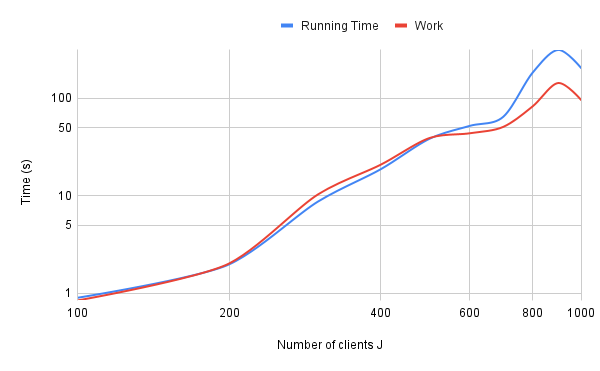
\includegraphics[width=.9\linewidth]{./chart.png}
\caption{Plotting in logarithm scale of execution time by number of clients.}
\end{figure}

As of work time, we can see in the Figure 1 that we have an exponential relationship between number of client and work/running time.

We do note the number of variables is proportional to the number of clients and we did not put the non-negativity constrains in the total number of constrains.

Also, we can note some weirdness in our data: the randomness of the instances made the instances with \(700\) an \(800\) clients have out of proportion result value, compared to its peers; we also note the execution time of the instance with \(900\) clients, which came out to be a lot slower than others. We do believe that anomaly maybe caused by some external factors involving the machine.
\end{document}
